%%%%%%%%%%%%%%%%%%%%%%%%%%%%%%%%%%%%%%%%%
% Jacobs Landscape Poster
% LaTeX Template
% Version 1.0 (29/03/13)
%
% Created by:
% Computational Physics and Biophysics Group, Jacobs University
% https://teamwork.jacobs-university.de:8443/confluence/display/CoPandBiG/LaTeX+Poster
% 
% Further modified by:
% Nathaniel Johnston (nathaniel@njohnston.ca)
%
% This template has been downloaded from:
% http://www.LaTeXTemplates.com
%
% 
% Masaryk University presentation themes were downloaded from:
% https://www.overleaf.com/gallery/tagged/muni
%
% and ported into Jacobs Landscape Poster by:
% Jumaidil Awal (ideal1st.here@googlemail.com)
% 
% Jacobs Landscape Poster License:
% CC BY-NC-SA 3.0 (http://creativecommons.org/licenses/by-nc-sa/3.0/)
%
% Masaryk University's fibeamer theme license:
% Copyright 2015  Vít Novotný <witiko@mail.muni.cz>
% Faculty of Informatics, Masaryk University (Brno, Czech Republic)
% under Latex Project Public License
%
%%%%%%%%%%%%%%%%%%%%%%%%%%%%%%%%%%%%%%%%%

%----------------------------------------------------------------------------------------
%	PACKAGES AND OTHER DOCUMENT CONFIGURATIONS
%----------------------------------------------------------------------------------------

\documentclass[final]{beamer}

\usepackage[scale=1.24]{beamerposter} % Use the beamerposter package for laying out the poster

%\usetheme{confposter} % Use the confposter theme supplied with this template
\usetheme[faculty=chemo]{fibeamer} % Uncomment to use Masaryk University's fibeamer theme instead.

% \setbeamercolor{block title}{fg=nred,bg=white} % Colors of the block titles
% \setbeamercolor{block body}{fg=black,bg=white} % Colors of the body of blocks
%\setbeamercolor{block alerted title}{fg=white,bg=dblue!70} % Colors of the highlighted block titles
%\setbeamercolor{block alerted body}{fg=black,bg=dblue!10} % Colors of the body of highlighted blocks
% Many more colors are available for use in beamerthemeconfposter.sty

%-----------------------------------------------------------
% Define the column widths and overall poster size
% To set effective sepwid, onecolwid and twocolwid values, first choose how many columns you want and how much separation you want between columns
% In this template, the separation width chosen is 0.024 of the paper width and a 4-column layout
% onecolwid should therefore be (1-(# of columns+1)*sepwid)/# of columns e.g. (1-(4+1)*0.024)/4 = 0.22
% Set twocolwid to be (2*onecolwid)+sepwid = 0.464
% Set threecolwid to be (3*onecolwid)+2*sepwid = 0.708

\newlength{\sepwid}
\newlength{\onecolwid}
\newlength{\twocolwid}
\newlength{\threecolwid}
\setlength{\paperwidth}{46.8in} % A0 width: 46.8in
\setlength{\paperheight}{33.1in} % A0 height: 33.1in
\setlength{\sepwid}{0.024\paperwidth} % Separation width (white space) between columns
\setlength{\onecolwid}{0.21\paperwidth} % Width of one column
\setlength{\twocolwid}{0.451\paperwidth} % Width of two columns
\setlength{\threecolwid}{0.678\paperwidth} % Width of three columns
%\setlength{\topmargin}{-0.5in} % Reduce the top margin size
%-----------------------------------------------------------

\usepackage{graphicx}  % Required for including images

\usepackage{booktabs} % Top and bottom rules for tables

%----------------------------------------------------------------------------------------
%	TITLE SECTION 
%----------------------------------------------------------------------------------------

\title{Neural mechanisms of risk-sensitive choice and reinforcement
learning under uncertainty} % Poster title

\author{Jan, Emil, Oguz, Vlad, Stephan Tietz} % Author(s)

\institute{Neural Information Processing Group, TU Berlin} % Institution(s)

%----------------------------------------------------------------------------------------

\begin{document}
\addtobeamertemplate{block end}{}{\vspace*{2ex}} % White space under blocks
\addtobeamertemplate{block example end}{}{\vspace*{2ex}} % White space under example blocks
\addtobeamertemplate{block alerted end}{}{\vspace*{2ex}} % White space under highlighted (alert) blocks

\setlength{\belowcaptionskip}{2ex} % White space under figures
\setlength\belowdisplayshortskip{2ex} % White space under equations
%\begin{darkframes} % Uncomment for dark theme, don't forget to \end{darkframes}
\begin{frame} % The whole poster is enclosed in one beamer frame

%==========================Begin Head===============================
  \begin{columns}
   \begin{column}{\linewidth}
    \vskip1cm
    \centering
    \usebeamercolor{title in headline}{\color{fg}\Huge{\textbf{\inserttitle}}\\[0.5ex]}
    \usebeamercolor{author in headline}{\color{fg}\Large{\insertauthor}\\[1ex]}
    \usebeamercolor{institute in headline}{\color{fg}\large{\insertinstitute}\\[1ex]}
    \vskip1cm
   \end{column}
   \vspace{1cm}
  \end{columns}
 \vspace{1cm}

%==========================End Head===============================

\begin{columns}[t] % The whole poster consists of three major columns, the second of which is split into two columns twice - the [t] option aligns each column's content to the top

\begin{column}{\sepwid}\end{column} % Empty spacer column

\begin{column}{\onecolwid} % The first column

%----------------------------------------------------------------------------------------
%	OBJECTIVES
%----------------------------------------------------------------------------------------

\begin{exampleblock}{Introduction}

\begin{itemize}
\item Mollis dignissim, magna augue tincidunt dolor, interdum vestibulum urna
\item Sed aliquet luctus lectus, eget aliquet leo ullamcorper consequat.
\end{itemize}

\end{exampleblock}

%----------------------------------------------------------------------------------------
%	INTRODUCTION
%----------------------------------------------------------------------------------------

\begin{exampleblock}{Background}
%TODO Change text about utility and risk sensitivites to a comic
%TODO Change text color of captions
%TODO Include information about exp UF and include the formula

\Large{Risk and Utility}

\normalsize

\begin{itemize}
    \item Risk is induced by choice with uncertain outcome.
    \item People behave \textbf{risk seeking}, \textbf{risk neutral} or \textbf{risk averse}.
    % \item Risk can exist without the danger of loss (e.g. loosing money).
    \item People map money to utility by \textbf{utility functions}, e.g. exponential utility $U(a) = (1-\exp(-\lambda a)) / \lambda$. 
    %\item The same amount of money can have different utility for different people.
    \item Curvature of function defines risk profile.
\end{itemize}

\hspace{2cm}


\newlength{\twosubht}
\newsavebox{\twosubbox}


\begin{figure}[htp]

% preliminary
\sbox\twosubbox{%
  \resizebox{\dimexpr.9\textwidth-1em}{!}{%
    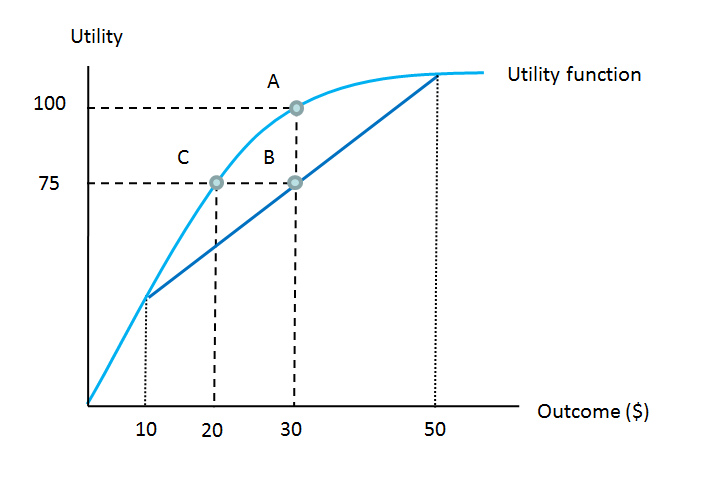
\includegraphics[height=10cm]{img/background/riskaversion}%
    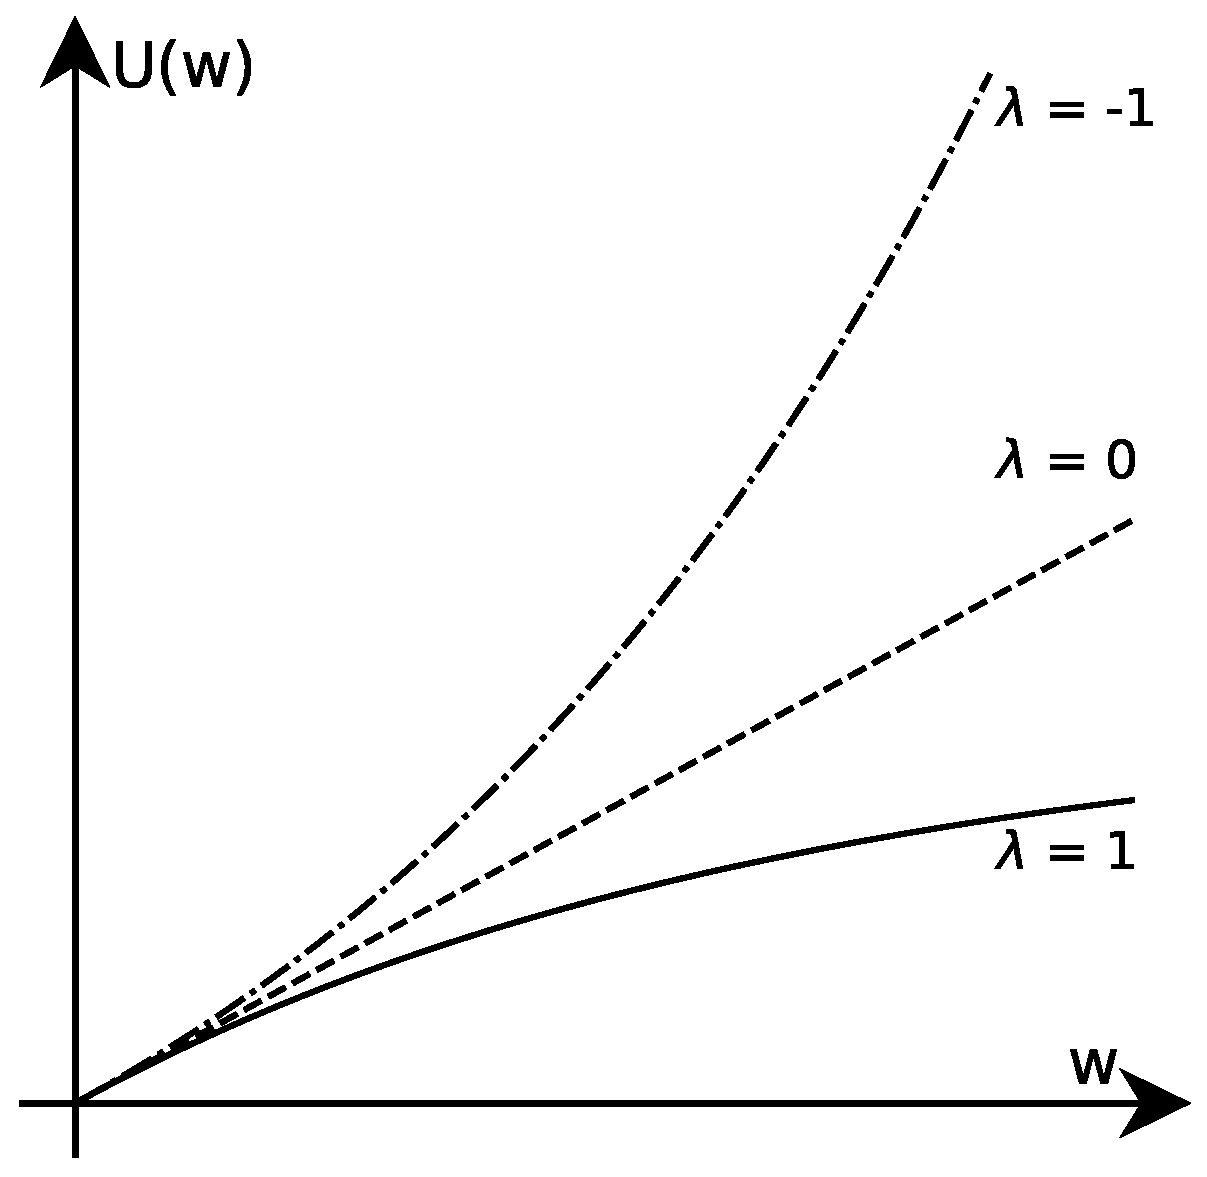
\includegraphics[height=10cm]{img/background/Exponential_Utility_Function}%
  }%
}
\setlength{\twosubht}{\ht\twosubbox}

% typeset

\centering

\subcaptionbox{Risk averse lottery\label{f}}{%
  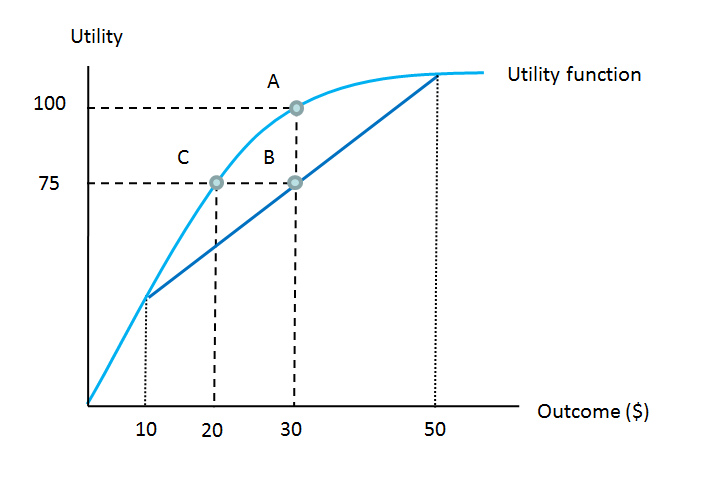
\includegraphics[height=\twosubht]{img/background/riskaversion}%
}\quad
\subcaptionbox{Exponential utility function\label{s}}{%
  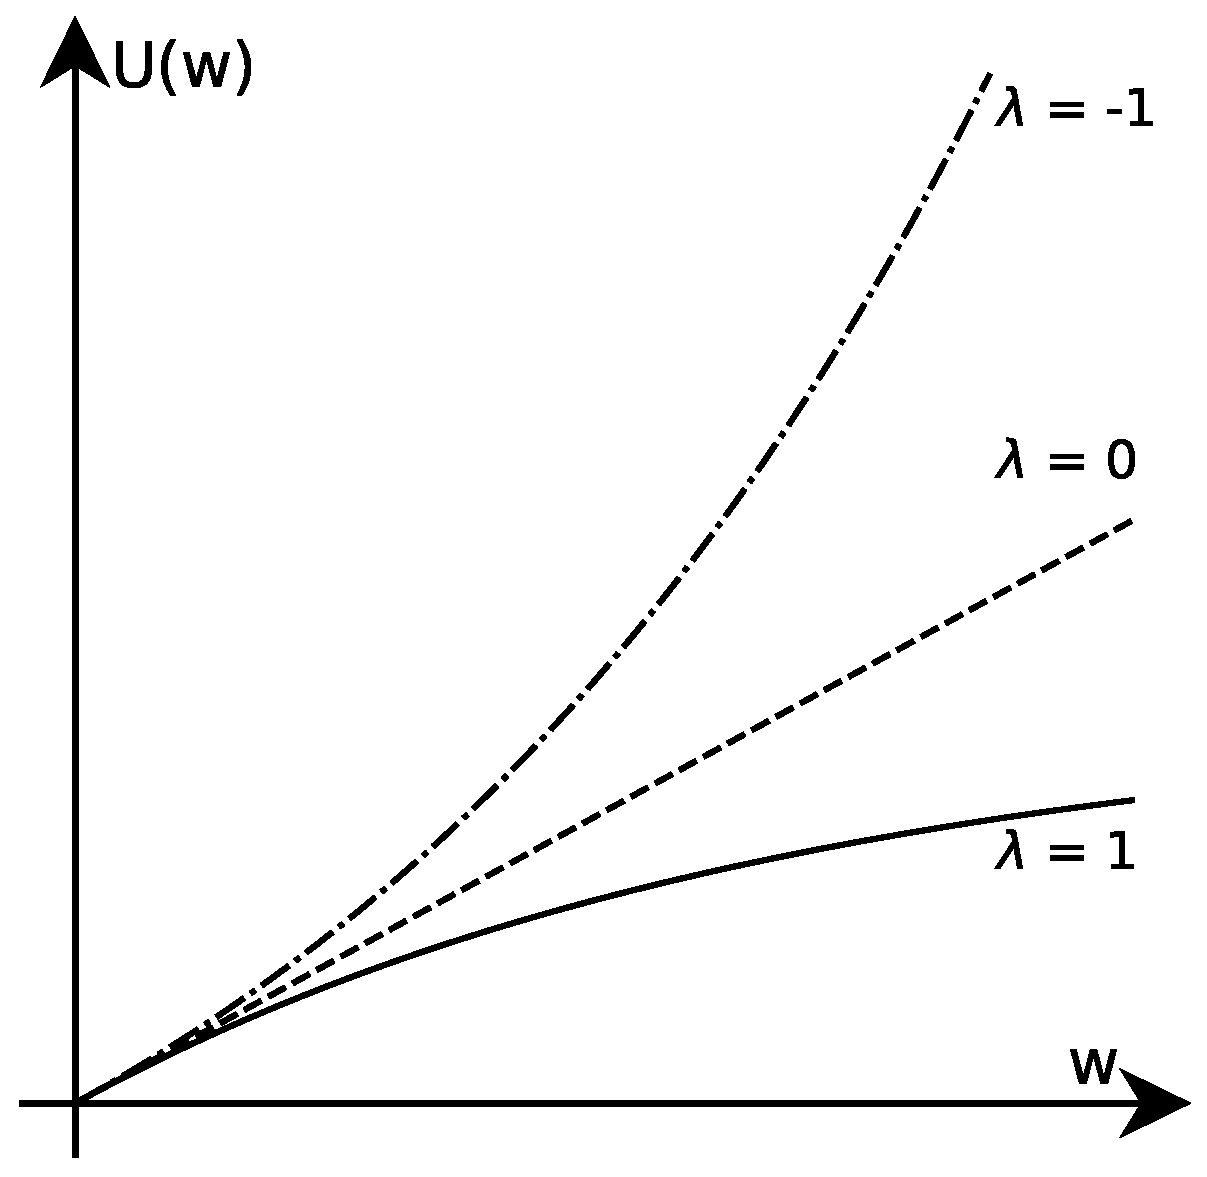
\includegraphics[height=\twosubht]{img/background/Exponential_Utility_Function}%
}

\caption{a) Choice from a risk free gift of 30\$ or a lottery where by coin flip you win 10\$ or 50\$. The utility for the risk free choice (point A) is higher than the expected utility of the risky lottery (point B). b) The exponential utility function for different risk parameters $\alpha$. $a < 0$ implies risk seeking, $a = 0 $ risk neutral and $a > 0 $ risk averse behaviour.}

\end{figure}


\Large{(Partially Observable) Markov Decision Process}

\normalsize
\begin{itemize}
    %\item Making decisions when state is not fully-observable.
    %\item Work on probability distribution over states rather than actual state.
    \item Current state not observable
    \item[$\rightarrow$] Estimate probability of state using observations
\end{itemize}

\hspace{2cm}


\begin{figure}
  \centering
    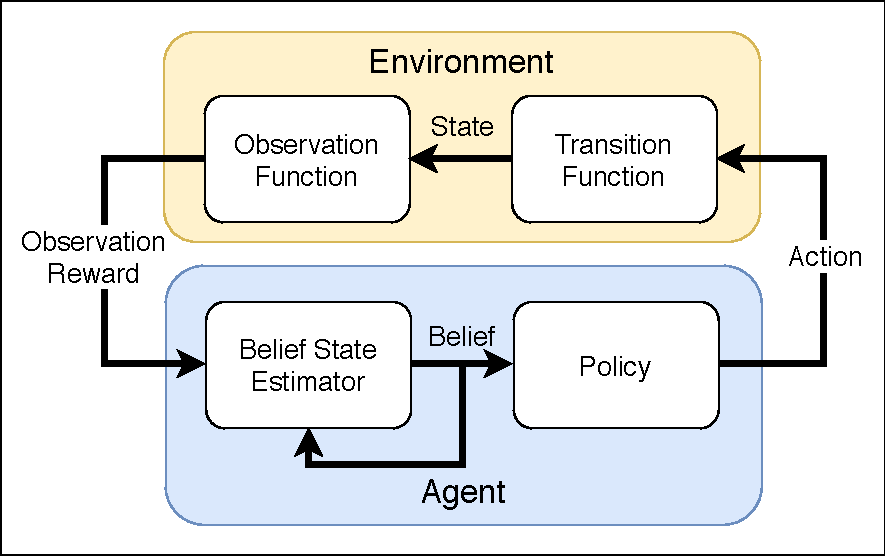
\includegraphics[width=0.7\textwidth]{img/background/POMDP}
  \caption{Sketch of a partially observable environment. The agent only gets observations as inputs.}
\end{figure}


%\begin{itemize}
%    \item Set of States $\mathcal{S}$ (Terminal and Non Terminal)
%    \item Set of Actions $\mathcal{A}$
%    \item Probabilistic Transitions depending on tuple $\mathcal{S} x \mathcal{A}$
%    \item Reward function $R(s,a)$
%\end{itemize}

%For partially observability states are hidden but produce observations:
%\begin{itemize}
%    \item Observation space $\mathcal{O}$
%    \item Observation function $p(o | s, a)$
%\end{itemize}

% add reference: http://www.cassandra.org/arc/papers/aaai94.pdf


\end{exampleblock}

%------------------------------------------------

\begin{figure}

\includegraphics[width=0.8\linewidth]{img/placeholder.jpg}
\caption{Figure caption}
\end{figure}

%----------------------------------------------------------------------------------------

\end{column} % End of the first column

\begin{column}{\sepwid}\end{column} % Empty spacer column

\begin{column}{\twocolwid} % Begin a column which is two columns wide (column 2)

\begin{columns}[t,totalwidth=\twocolwid] % Split up the two columns wide column

\begin{column}{\onecolwid}\vspace{-.74in} % The first column within column 2 (column 2.1)

%----------------------------------------------------------------------------------------
%	MATERIALS
%----------------------------------------------------------------------------------------

\begin{exampleblock}{Materials}

The following materials were required to complete the research:

\begin{itemize}
\item Curabitur pellentesque dignissim
\item Eu facilisis est tempus quis
\end{itemize}

The materials were prepared according to the steps outlined below:

\begin{enumerate}
\item Curabitur pellentesque dignissim
\item Eu facilisis est tempus quis
\end{enumerate}

\end{exampleblock}

%----------------------------------------------------------------------------------------

\end{column} % End of column 2.1
\begin{column}{\sepwid}\end{column} % Empty spacer column

\begin{column}{\onecolwid}\vspace{-.74in} % The second column within column 2 (column 2.2)

%----------------------------------------------------------------------------------------
%	METHODS
%----------------------------------------------------------------------------------------

\begin{exampleblock}{Methods}

Lorem ipsum dolor \textbf{sit amet}, consectetur adipiscing elit. Sed laoreet accumsan mattis. Integer sapien tellus, auctor ac blandit eget, sollicitudin vitae lorem. Praesent dictum tempor pulvinar. Suspendisse potenti. Sed tincidunt varius ipsum, et porta nulla suscipit et. Etiam congue bibendum felis, ac dictum augue cursus a. \textbf{Donec} magna eros, iaculis sit amet placerat quis, laoreet id est.

\end{exampleblock}

%----------------------------------------------------------------------------------------

\end{column} % End of column 2.2

\end{columns} % End of the split of column 2 - any content after this will now take up 2 columns width

%----------------------------------------------------------------------------------------
%	IMPORTANT RESULT
%----------------------------------------------------------------------------------------

\begin{alertblock}{Important Result}

Lorem ipsum dolor \textbf{sit amet}, consectetur adipiscing elit. Sed commodo molestie porta. Sed ultrices scelerisque sapien ac commodo. Donec ut volutpat elit.

\end{alertblock} 

%----------------------------------------------------------------------------------------

\begin{columns}[t,totalwidth=\twocolwid] % Split up the two columns wide column again

\begin{column}{\onecolwid} % The first column within column 2 (column 2.1)

%----------------------------------------------------------------------------------------
%	MATHEMATICAL SECTION
%----------------------------------------------------------------------------------------

\begin{exampleblock}{Mathematical Section}

Nam quis odio enim, in molestie libero. Vivamus cursus mi at nulla elementum sollicitudin. Nam quis odio enim, in molestie libero. Vivamus cursus mi at nulla elementum sollicitudin.
  
\begin{equation}
E = mc^{2}
\label{eqn:Einstein}
\end{equation}

\begin{equation}
\cos^3 \theta =\frac{1}{4}\cos\theta+\frac{3}{4}\cos 3\theta
\label{eqn:cosfunc}
\end{equation}

Nam quis odio enim, in molestie libero. Vivamus cursus mi at nulla elementum sollicitudin. Nam quis odio enim, in molestie libero. Vivamus cursus mi at nulla elementum sollicitudin.

\begin{equation}
\kappa =\frac{\xi}{E_{\mathrm{max}}} %\mathbb{ZNR}
\label{eqn:kappa}
\end{equation}

\end{exampleblock}

%----------------------------------------------------------------------------------------

\end{column} % End of column 2.1
\begin{column}{\sepwid}\end{column} % Empty spacer column

\begin{column}{\onecolwid} % The second column within column 2 (column 2.2)

%----------------------------------------------------------------------------------------
%	RESULTS
%----------------------------------------------------------------------------------------

\begin{exampleblock}{Results}

\begin{figure}

\includegraphics[width=0.8\linewidth]{img/placeholder.jpg}
\caption{Figure caption}
\end{figure}

Nunc tempus venenatis facilisis. Curabitur suscipit consequat eros non porttitor. Sed a massa dolor, id ornare enim:

\begin{table}
\vspace{2ex}
\begin{tabular}{l l l}
\toprule
\textbf{Treatments} & \textbf{Response 1} & \textbf{Response 2}\\
\midrule
Treatment 1 & 0.0003262 & 0.562 \\
Treatment 2 & 0.0015681 & 0.910 \\
Treatment 3 & 0.0009271 & 0.296 \\
\bottomrule
\end{tabular}
\caption{Table caption}
\end{table}

\end{exampleblock}

%----------------------------------------------------------------------------------------

\end{column} % End of column 2.2

\end{columns} % End of the split of column 2

\end{column} % End of the second column

\begin{column}{\sepwid}\end{column} % Empty spacer column

\begin{column}{\onecolwid} % The third column

%----------------------------------------------------------------------------------------
%	DISCUSSION
%----------------------------------------------------------------------------------------

\begin{exampleblock}{Discussion}

\begin{itemize}
    \item Exponential utility function p
\end{itemize}

\end{exampleblock}

%----------------------------------------------------------------------------------------
%	ADDITIONAL INFORMATION
%----------------------------------------------------------------------------------------

\begin{exampleblock}{Additional Information}

Maecenas ultricies feugiat velit non mattis. Fusce tempus arcu id ligula varius dictum. 
\begin{itemize}
\item Curabitur pellentesque dignissim
\item Eu facilisis est tempus quis
\item Duis porta consequat lorem
\end{itemize}

\end{exampleblock}

%----------------------------------------------------------------------------------------
%	REFERENCES
%----------------------------------------------------------------------------------------

\begin{exampleblock}{References}

\nocite{*} % Insert publications even if they are not cited in the poster
\small{\bibliographystyle{unsrt}
\bibliography{sample}\vspace{1cm}}
\end{exampleblock}

%----------------------------------------------------------------------------------------
%	ACKNOWLEDGEMENTS
%----------------------------------------------------------------------------------------

%\setbeamercolor{block title}{fg=red,bg=white} % Change the block title color

%\begin{exampleblock}{Acknowledgements}

%\small{\rmfamily{Nam mollis tristique neque eu luctus. Suspendisse rutrum congue nisi sed convallis. Aenean id neque dolor. Pellentesque habitant morbi tristique senectus et netus et malesuada fames ac turpis egestas.}} \\

%\end{exampleblock}

%----------------------------------------------------------------------------------------
%	CONTACT INFORMATION
%----------------------------------------------------------------------------------------

%\setbeamercolor{block alerted title}{fg=black,bg=norange} % Change the alert block title colors
%\setbeamercolor{block alerted body}{fg=black,bg=white} % Change the alert block body colors

\begin{block}{Contact Information}

\begin{itemize}
\item Web: \href{http://ideal1st.com/}{http://ideal1st.com/}
\item Email: \href{mailto:ideal1st.here@gmail.com}{ideal1st.here@gmail.com}
\end{itemize}

\end{block}

\begin{tabular}{rr}
\hspace{0.3\linewidth} & 
\includegraphics[width=0.7\linewidth]{img/chemo-kamen-normal-mode.png}
\end{tabular}

%----------------------------------------------------------------------------------------

\end{column} % End of the third column

\begin{column}{\sepwid}\end{column} % Empty spacer column

\end{columns} % End of all the columns in the poster

\end{frame} % End of the enclosing frame
%\end{darkframes} % Uncomment for dark theme
\end{document}
